%%%%%%%%%%%%%%%%%%%%%%%%%%%%%%%%%%%%%%%%%%%%%%%%%%%%%%%%%%%
%
% Using the same LaTeX template as Brooke Simmons HST Proposal.
% This is used in HST applications with STScI.
% PHASE I: Archival & Theoretical Research Proposal Template
%
% I'm open to changing the proposal template.

\documentclass[11pt,usenatbib]{article}
\usepackage{phase1}
\usepackage{wrapfig}
\usepackage{caption}
\usepackage{graphicx, graphics}
\usepackage{enumitem}
\usepackage[utf8]{inputenc}
\usepackage[T1]{fontenc}
\usepackage{natbib}
\usepackage{hyperref}
\usepackage{ae,aecompl}
\usepackage{color}

\title{ESA Fellowship Proposal: Statistically Constraining the Interacting Galaxy Population}
\author{David O'Ryan}

\definecolor{titlecol1}{rgb}{0.7,0.0,0.05} %dark red
\definecolor{titlecol2}{rgb}{0.039,0.361,0.569} %teal++

\begin{document}
    \begin{center}
        \large{{ESA Fellowship Proposal: Linking Galaxy Morphology with Parameterisation and Their Physical Processes \\
        Potential Fellow: David O'Ryan \\
        Potential Mentor(s): Bruno Alteiri \& Bruno Merin}}
    \end{center}
    
% \vspace{-7mm}
% \begin{abstract}
% \vspace{-3.5mm}
% Relating the fundamental parameters of galaxies to a multitude of underlying processes and their morphology is a notoriously difficult task. Often, data containing fully parameterised galaxies is sparse (or concentrated in specific areas of the sky) while morphological classification data of galaxies is limited. Rarely do these sets of data overlap. The result of this is that we have a complete disconnect between investigating the morphological relationship of galaxies with their parameterisation. By using the newly released convolutional network \texttt{Zoobot} from the Galaxy Zoo collaboration and the recently launched Euclid observatory, I will rectify this. I will create the largest catalogue of morphologically classified galaxies with complete ancillary data to date. This catalogue will be similar to the COSMOS catalogue, but across the entire sky. We will conduct initial analysis of this catalogue before releasing it to the community for further use. We will conduct initial analysis of this catalogue, linking a multitude of parameters with morphology, and inferring links between underlying physical processes within galaxies to their parameters and morphology. We will also conduct in depth analysis of a specific galaxy type in this catalogue to show its power: interacting galaxies. 
% \end{abstract}

\vspace{-5mm}
\justification
\vspace{-3mm}
\noindent\textbf{Linking Galactic Morphology with Photometric Parameterisation} \\
Photometric parameterisation of galaxies is nothing new in the field of astrophysics. By measuring specific emission lines in galaxies, it is possible to conduct spectral energy distribution (SED) fitting to infer their masses, star formation rates, etc. This allows us to make interesting links between physical processes occurring within them. An example of such a catalogue that has seen much use over the last fifteen years is the COSMIC Evolution Survey (COSMOS) \citep{cosmos catalogue}. This catalogue contained the measured emission lines of 1.7 million galaxies in a 3$^{\circ} \times $3$^{\circ}$ area of the sky. Not only does it contain their emissions, but also their parameterisations (stellar masses, luminosities, photometric redshifts, star formation rates, etc) calculated by the COSMOS team. This catalogue has therefore been used in multiple papers (at time of writing, easily 1000+) to investigate the properties of different types of galaxies. These different types can be interacting galaxies, spiral galaxies, elliptical galaxies, barred galaxies, etc.

The key to understanding the relationship between different types of galaxies and the processes within them is to have statistically significant samples of galaxies. While 1.7 million is certainly statistically significant in itself, it is over X\% of the sky. Also, once we start to split these 1.7 million into the multiple kinds of galaxies we want to investigate, we begin to lose that statistical completeness. Often users will have existing catalogues of a type of galaxy they want to investigate which only partially overlaps with the area COSMOS covers. (need to give examples here). Therefore, much of a specific sample does not have their parameters available for them for full investigation and cannot be used. This can be particulary true when linking galaxy parameterisation to morphology.

Large catalogues of galaxy morphology are beginning to come into existence, often thanks to the Galaxy Zoo Collaboration \citep{lintott_08}. This has allowed for many interesting results and insights into the formation of different galaxy morphologies. However, the overlap between morphology catalogues and ancillary data of parameterisation are often limited. A powerful example was that of the Galaxy Zoo: COSMOS project \citep{}, where Galaxy Zoo specifically targeted galaxies within the COSMOS field. This sudden overlap between them lead to many publications and linking of specific structures in galaxies to their parameters. A prime example is that of nuclear activity in galaxies with existing strong or weak bars \citep{papers using cosmos with galaxy zoo}. Thus, it is not enough to simply have identified galaxy morphology without additional ancillary data or vice versa. We must also have the ancillary data to extrapolate and explore the underling parameter space. We need spectra of them to prove to fit SED templates to to measure their masses or to measure their star formation rates. 

This project will focus on bridging this gap. We will utilise the newly released ESA Datalabs to fully explore the \texttt{Hubble} archives and morphologically classify every galactic source within it. This will be done using the newly released convolutional neural network (CNN) \texttt{Zoobot} \citep{Zoobot paper} from the Galaxy Zoo Collaboration. \texttt{Zoobot} is trained to classify galaxies in a similar manner to citizen scientists themselves. It is trained to answer all classification questions simultaneously, giving robust morphological classifications to each source whose error can investigated directly. We will combine this approach with the all-sky spectroscopic survey of the newly launched Euclid observatory. As this data becomes available, we will create the largest catalogue of galaxies with ancillary data to date. We will also enhance this catalogue by parameterising each galaxy from its spectroscopic information. This will be done using existing, and well used, astrophysical fitting software. The many options are: Easy and Accurate zPhot from Yale (EAzY; \citet{Brammer et al. 2008}) followed by the Fitting and Assessment of Synthetic Templates (FAST; \citet{Kriek et al 2009}), Photometric Analysis for Redshift Estimate (LePHARE; \citet{Arnouts et al. 1999, Ilbert et al. 2006}) or Multi-Wavelength Analysis of Galaxy Physical Properties (MAGPHYS; \citet{da Cunha et al. (2008)}).

Once this catalogue is created, we will conduct an initial analysis and explore the underlying parameter space of a multitude of galaxy types. Another power of this approach is that we will discover, in the archives, a multitude of objects of significant astrophysical interest. Many of these object types, we only have a few dozen to a few hundred examples in the literature. These galaxy types are: jellyfish galaxies, interacting galaxies, galaxy groups, edge-on proto-planetary disks, etc.

In the next section, I will detail how I will leverage the \texttt{Hubble} archives to find large, statistically robust samples of a multitude of objects of astrophysical interest. I will describe how my existing experience with ESA Datalabs, as well as with the CNN \texttt{Zoobot} will allow me to quickly deliver these catalogues to the community. In section 3, I will discuss how an initial exploration of combining the COSMOS catalogue an existing catalogue from ESA Datalabs shows the potential for this project. I will then describe how I will exploit the ancillary data as it comes in from Euclid to conduct initial statistical analysis on various galaxies. Finally, I will discuss a side project, where I will use software I have built in my PhD to completely explore the underlying parameter space of interacting galaxies by directly using observation.
\\
\\
\noindent \textbf{Creating Statistically Robust Galaxy Samples with ESA Datalabs} \\
As shown in my first paper \citep{O'Ryan}, it is possible to create extremely large catalogues of different astrophysical objects even under very conservative conditions. In that project, we utilised the CNN \texttt{Zoobot} in conjunction with direct access to the \textt{Hubble} Science Archives via ESA Datalabs. The resultant catalogue of 21,926 interacting galaxies was the largest catalogue of interacting galaxies at the time of publication. However, in making such a catalogue (in such a short timeframe) certain sacrifices had to be made. First, there are multiple issues with identifying interacting galaxies by visualisation alone. Often contamination by close pairs (i.e. galaxies close together by projection effects on the sky, not actually interacting) outweight any interacting galaxies found. This collapse of purity often makes seemingly large, statistically robust, catalogues useless. Therefore, in this project we focused on interacting galaxies which specifically had tidal features; focusing the CNN on classifying them. This focuses the catalogue on a specific timeframe of interaction. The second sacrifice was that of purity over completeness. We used incredibly conservative classification criteria when defining an interacting galaxy - due to the problem of close pairs. This means that may real interacting galaxies will have been misidentified as non-interacting.

However, what this project demonstrated was the capability of leveraging the archives to make the largest possible catalogues of astrophysical objects of interest to date. Not only did I find interacting galaxies with this approach, but also a whole host of other objects in the contamination of the final catalogue. Therefore, if given the opporunity, I would expand this project significantly. With further upgrades to \texttt{Zoobot} since I used it, it's accuracy for this task has dramatically improved. While I would focus on releasing a complete catalogue of interacting galaxies (and calculating that completeness) I would also release catalogues of many different kinds and morphologies of galaxies. There are many astrophysical objects which we only have a few dozen examples. By leveraging the archives, I would expand those catalogues by an order of magnitude - as I did for interacting galaxies.

The key difference between the project I propose here and the internship I conducted is the shift in focus to analysis and followup. This project will be conducted at a time where Euclid will begin taking data, the James Webb Space Telescope (JWST) has already obtained a treasure trove of data and the development of ESA Datalabs is nearing its completion. Because of my experience with ESA Datalabs and the archives when their development was only just beginning, I m well suited to take advantage of these tools immediately and get quick returns on their deployment. The only barrier to me, currently, is that I am not in the Euclid consortium to take immediate access of the data. However, if this application progresses, I will begin the process of joining it so I can access and utilise their data. This will be paramount, as the second focus of this proposal is to begin anaylsis of the objects we find through the archives. This requires ancillary data. That ancillary data will come from Euclid, and the softwares described previously. The power of this combination is already becoming apparent, with the investigation of the \citet{O'Ryan} catalogue using the COSMOS field. This case study is explained in the next section, and then the full scope of this project revealed.
\\
\\
\noindent \textbf{The Success of the COSMOS Catalogue and the Potential of Euclid} \\
An example of value adding to the catalogues that will come out from the archives is that of comparing my \citet{O'Ryan} catalogue to the COSMOS catalogue. COSMOS is a catalogue of ancillary data. It contains the coordinates of over 1.7 million sources (the COSMOS2020 Classic catalogue does), as well as observed magnitudes and emissions from each. The true value then comes from the catalogue team applying the previously described softwares to their sources. This allows them to also publish, with the observations and source coordinates, estimates of photometric redshifts, estimates of stellar masses, star formation rates, etc. These can then be used to infer relations between the types of galaxies and their parameters.

We conducted a matching between COSMOS and the \citet{O'Ryan} catalogue purely on source coordinates, and recovered 3,897 matches. We were also able to recover the secondary galaxies in each of these systems, giving us ancillary data to a total of 7,794 interacting galaxies. While this analysis is only just coming to its conclusion, the prelimary results are fascinating. By breaking down each system into a different stage of interaction, we had found direct links between that and the star formation rates observed in them. We are also relating the stages to AGN activity, finding activation begins to occur in a specific stage. These results are shown in figure \ref{fig:comsos_results}.

\begin{figure}
    \centering
    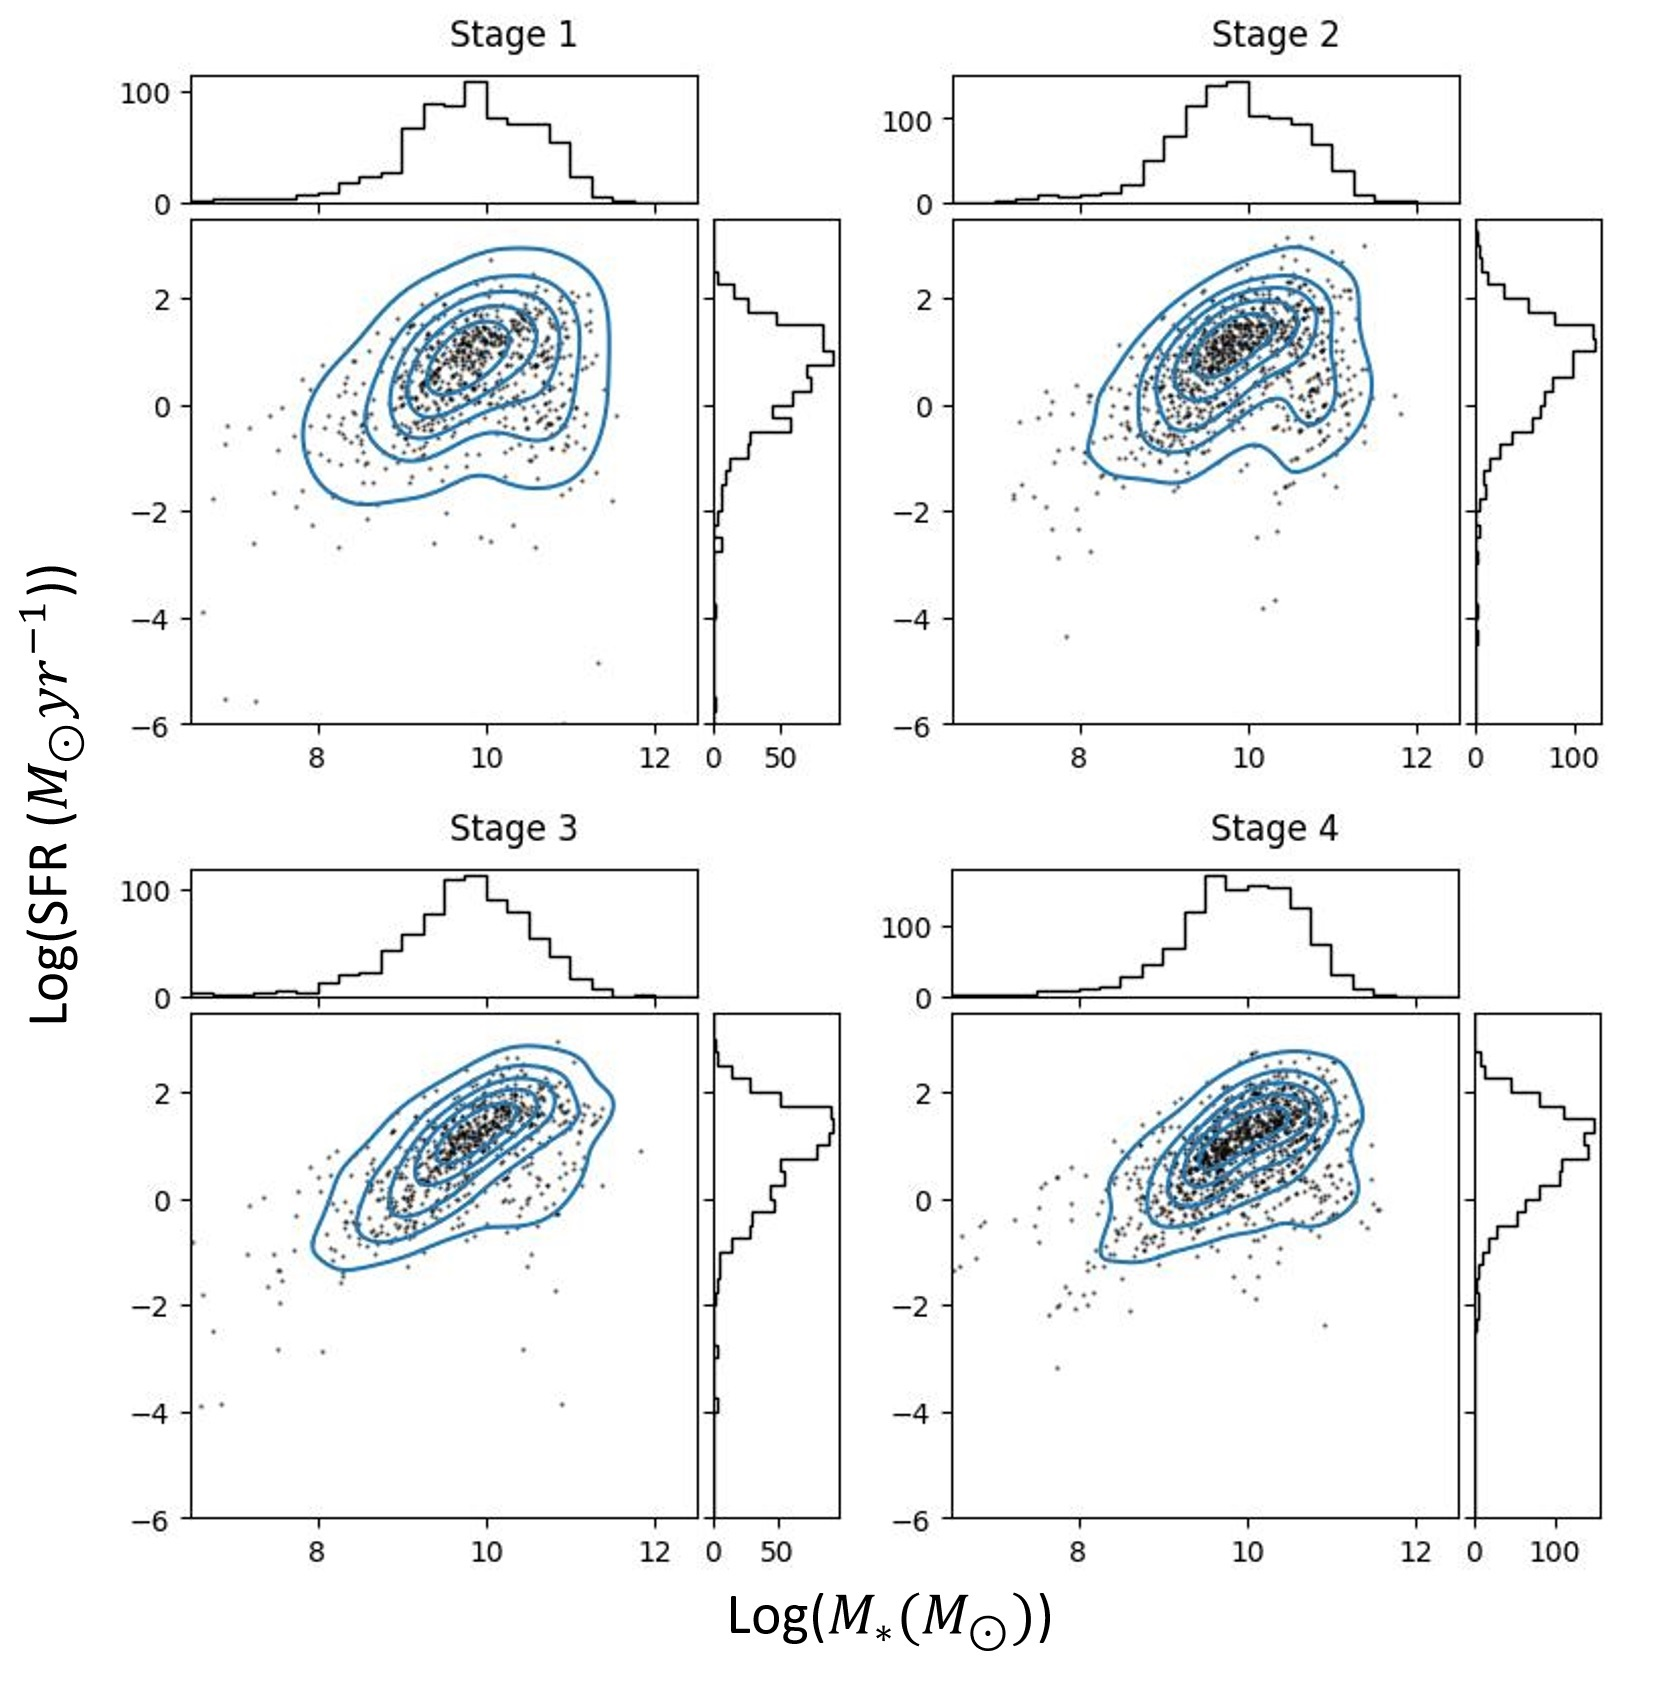
\includegraphics[width=\textwidth]{figures/stage-evol.jpg}
    \caption{Initial results of combining the \citet{O'Ryan} catalogue with the ancillary data of the COSMOS catalogue. Each interaction has been broken up into different stages of interaction, and their stellar masses and star formation rates plotted. In stages 1 and 2, we see that there is a secondary population of high mass, lower star forming galaxies which disappears as we move into stages 3 and 4 of the interaction. This is shown best by the contours in each subplot, but can also be observed in the slope of the histograms. This is evidence of when a starburst may occur in interacting systems through an interaction, an important pieve of evidence we are missing in understanding the effects of interaction on the galactic population.}
    \label{fig:cosmos-label}
\end{figure}

Now, these discoveries and inferences are coming from a fifth of the interacting galaxies in the \citet{O'Ryan} catalogue. This is simply a fact of those galaxies which overlap with the COSMOS field. However, Euclid will allow us to bring a completely new scale to this approach. While the observing area of the COSMOS field is relatively small (approximately $3^{\circ} \times 3^{\circ}$) Euclid will be an all sky survey mission. Not only could the entirety of the \citet{O'Ryan} catalogue be covered by Euclid, and ancillary data created for it, but any objects of astrophysical interest throughout other catalogues we find will have ancillary data available.

Thus, this project will aim to combine the approaches of the Galaxy Zoo and COSMOS collaborations. The specific relating of galactic parameters (stellar masses, sizes, environment, etc) to physical processes (star formation, nuclear ignition, bar formation, etc) is poorly understood and constrained. The connection between such parameters and morphology is a further complication. Often, it is impossible to directly investigate both morphology and parameterisation simultaneously due to a lack of overlap between the data. In this project, we will be creating both sets of data for every object in the \texttt{Hubble} archives which is also overlapped by Euclid. Before doing any analysis, I predict the usefulness of these catalogues will be huge in the community. For reference, the first Galaxy Zoo paper \citep{lintott_08} has 806 citations while the initial COSMOS catalogue data release has 695 citations. Therefore, the potential impact of releasing a combined catalogue, before we conduct any fundamental analysis, of morphological and galactic parameterisation is colossal.
\\
\\
\noindent \textbf{Aside: Parameterisation of Interacting Galaxies} \\
\noindent While the focus of this project will be on creating and analysing the results of statistically robust, ancillary complete catalogues of all kinds of galaxies a special focus will be given to interacting galaxies. My PhD project has been focused on constraining galaxy interaction by directly comparing simulations to observations. The aim has been to parameterise the galaxies involved in the interaction and relate those parameters to the tidal features that form in the interaction. Initial results found by comparing to those from Galaxy Zoo: Mergers project will soon be pulished, showing the viability of this approach. The approach utilises an efficient N-body interaction modeller with Markov-Chain Monte Carlo methods to fully explore a pre-defined parameter space and show the parameter values that have the highest probability of forming those tidal features. The limitation of this, in my PhD, was that this approach was only applied to a sample of sixty interacting galaxies: hardly a statistically significant sample. 

Using the catalogues generated here, interacting galaxies will be identified (similar to in \citet{O'Ryan}). However, using Euclid they will also be spectroscopically confirmed. This will give us a sample of high purity and completeness, eradicating the problem of close pairs entirely. I will then apply the methods developed in my PhD to this sample, and demonstrate an initial use of the catalogues we are creating. I will fully statistically constrain which areas of parameter space of interaction lead to the formation of tidal features for the full population of interacting galaxies. As the work developing this code has been completed in my PhD, I will simply have to apply it to the resulting catalogues of this project to investigate this. 

\vspace{-3mm}
\describearchival
\vspace{-3mm}
\noindent\textbf{Project Timeline \& Project Results} \\
\noindent The timeline described in this section assumes a project timescale of 3 years and is laid out as shown in Fig \ref{fig:gantt-chart}. Each specific part of the project has been broken down into different work packages (WP) and then broken down into tasks to be completed. The definition of of each work package, and the tasks involved is explained below.

\begin{figure}
    \centering
    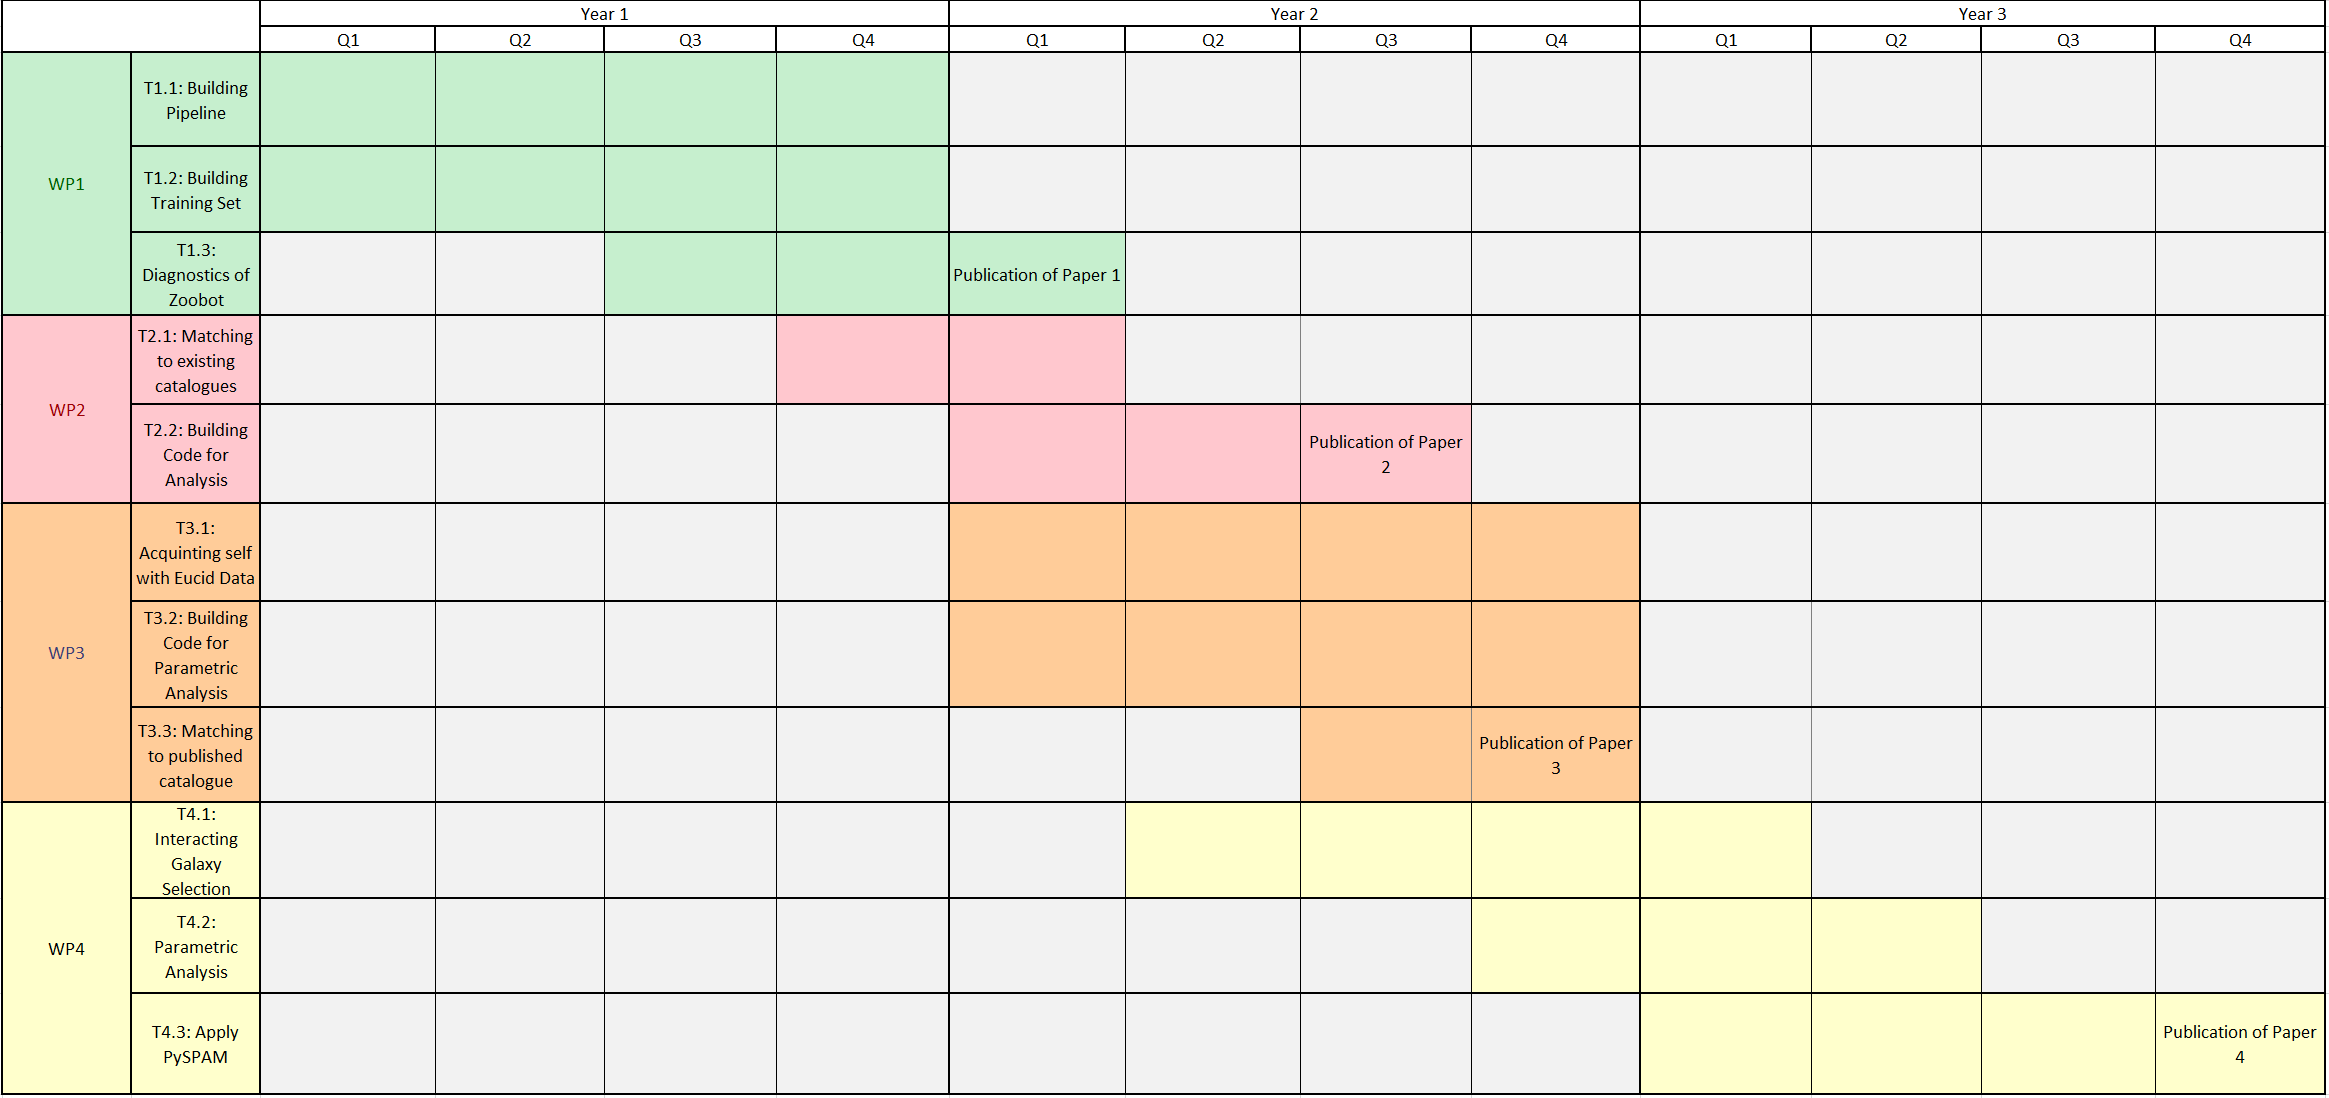
\includegraphics[width = \textwidth]{figures/draft-gantt.png}
    \caption{GANTT chart detailing the timelines planned for the four Work Packages defined in this proposal. As shown, it is expected that four distinct papers will be published from this project, primarily detailing new catalogues with incredibly useful ancillary data for the community. The final paper will be a direct demonstration of the power of these catalogues using them to investigate and statistically constrain interacting galaxies.}
    \label{fig:gantt-chart}
\end{figure}

\noindent \textbf{WP 1: Building the Classification Pipeline, Training and Creating a Morphological Catalogue} In order to classify the morphology of greater than 126 millions sources, a robust pipeline will need to be built. This pipeline must be able to: create reasonable source cutouts in a general way, be able to identify bad cutouts, feed them into a trained classifier and be fully diagnostically checked before running on the full sample and classifying every source. In my internship at ESAC, this part was the bulk of the project. I, therefore, will be putting at least 4 quarters into this part. This work package will also include the writing up of a large data release as well as a breakdown of objects of interest found. This resultant paper will be analogous to \citet{O'Ryan}.

\noindent \textbf{WP 2: Analysing Morphological Classifications} Once the pipeline has been completed, and run upon all sources, excellent analysis can then be conducted involving the specific morphologies. What will be of intense interest to myself will be building a link here between the existence of morphological structures and environment. I will also aim to cross-match any sources found here with existing catalogues of ancillary data to link in photometric parameterisations. Therefore, I aim to build links, specifically, between environmental density, the formation of galactic structures (such as bars or spirals) and photometric galactic parameters (such as star formation rates and stellar mass).

\noindent \textbf{WP 3: Analysing Euclid Data and Creating Photometric Parameterisation} By the time the previous two WPs have been completed, the first few data releases from Euclid should be publicly available (or, at least, available within the consortium). I will spend the time here gauging the work required to build the ancillary catalogue to go with the morphological one. I will mess around with Euclid data, and investigate what reductions must be done with it. I will then utilise EAZY, LePhare and FAST to calculate photometric galaxy parameters of any overlapping data. I will then release this ancillary catalogue to the community. Assuming that there is sufficient overlap to build a statistically significant sample, I will investigate any links between environment, morphology and photometric parameters over this wider sample. At this stage, I will also begin to specifically select out interacting galaxies from the sample for WP 4.

\noindent \textbf{WP 4: Use Case of Catalogue: Interacting Galaxies} In the final WP, I shall conduct a deep dive on using the new catalogue of objects specifically with regard to interacting galaxy. Using this large sample of photometrically confirmed interacting galaxies, I will investigate relations between the photometric parameters, interaction stage, the tidal features formed, nuclear activity and star formation rate enhancement. I will also apply my own algorithm to this sample, and explore the full parameter space of interaction and find which parameters lead to specific tidal features.
\\
\\
% The first year of this project will primarily be focused on developing the code to extract excellent cutouts of all sources in the \texttt{Hubble} source catalogue. While I currently have the code to generate these cutouts from my internship, some refinements must be made. Specifically, the size of the cutout must be based upon the size of the source within it. This will ensure the source is fully resolved in the cutout; an issue discovered when keeping a fixed cutout size in the \citet{O'Ryan} catalogue. This time will also be used to test the accuracy of \texttt{Zoobot} through different \texttt{Hubble} filters and instruments. For these tests I will need to create training sets of different galaxies with full descriptions from Galaxy Zoo.

% Once the code is created and tested, it will be run on the entire \texttt{Hubble} archives across all filters and instruments. The classification will take some time. From the creation of the \citet{O'Ryan} catalogue, 92 million sources took approximately one month to classify. As we add further source catalogues or instruments into our pipeline, the classification process itself may take more than this. We therefore schedule in 2.5 months for this process. As this process continues, I will shift my focus to the secondary goals of this project. I will begin to investigate Euclid data and get acquainted with it. I will focus my attention on interacting galaxies and further constraining the \citet{O'Ryan} catalogue. I will also have access to the results as they come in, allowing me to investigate the results and make some preliminary investigations into what we might find. I will also begin building the pipeline that will utilise the ancillary data to compute each galaxies parameterisation.

% Finally, in the third year of this project, I will conduct the key analysis of the full catalogue we create. I will present an initial review of the parameter space we have covered as well as the limitations of the catalogue. I will the conduct an investigation into the different types of galaxies vs the parameterisations we have made. I will pick out the interacting galaxies for an example paper of how to use the catalogue, and do a in-depth exploration of their parameter space. To finalise the project, I will conduct my own analysis of the new interacting galaxy sample and apply the software developed in my PhD to completely match the underlying parameter space to tidal features that form. \\

%%%% Rewrite above, but put it in terms of Work Packages with specific goals. 
% Work Package 1: Building the pipeline that will conduct the classifications of the objects.
% Work package 2: Analysing the resultant data from all objects in HSC. Also diagnosing model completeness, purity, etc.
% Work Package 3: Combining with Ancillary data from Euclid. This includes checking Euclid data and applying photometric algorithms.
% Work Package 4: Deep dive on interacting galaxies and conducitng their full parameterisation.

\noindent\textbf{Expected Science Results} \\
\noindent Here, we describe the specific scientific outputs expected from each WP. Currently, they are simply the names of the papers expected, but can be expanded upon further on request. From the four work packages, I anticipate that there will be five scientific publications. The titles of these will be:

\begin{enumerate}[itemsep=0pt, parsep=0pt, topsep=0pt]
    \item \textbf{WP1}: A Complete Sample of Interacting Galaxies: An Initial Exploration
    \item \textbf{WP1}: A Morphological Catalogue of 126 Million Sources from the Hubble Source Catalogue
    \item \textbf{WP2}: Combining Morphology and Parameterisation: A Morphology Catalogue Matched to COSMOS
    \item \textbf{WP3}: Linking Morphology and Euclid: A Catalogue of N Galaxies with full Morphological and Ancillary
    \item \textbf{WP3} Leveraging Parameterisation: A Statistical Study Linking Galaxy Parameters to Galaxy Types
    \item \textbf{WP4} Exploring the Interacting Galaxy Population: Linking Underlying Parameters to Feature Formation
\end{enumerate}

\noindent On top of these, I will also aim to publish two further works on what we find in the archives. These will be relatively short, low hanging fruit papers which provide coordinates and classifications of rare astrophysical objects to the community:
\begin{enumerate}[itemsep=0pt, parsep=0pt, topsep=0pt]
    \item \textbf{WP1.1}: The Gems of the Archives: Release of a Catalogue of Rare Galaxy Types from the \texttt{Hubble} Archives
    \item \textbf{WP4.1}: Directly Investigating Interaction: Exploring the Underlying Parameter Space of a Statistically Robust Sample of Interacting Galaxies
\end{enumerate}

% See how I did this in the FlatIron proposal. And then we've just got to make the damn thing fit. 
% Fit, re-read and then make sure we have everything!
% \noindent \textbf{References}\\
% {}

\bibliographystyle{mnras}
\bibliography{References}

\end{document}